% Fig. 4.15 -- 二元常態聯合 pdf 的立體鐘形，兩面板。
% 書稿來源: mathstatch4.tex 第 5219 至 5267 行 (左面板) 與第 5270 至 5319 行
%   (右面板)。書稿把兩個 tikzpicture 各放進一個 .49\textwidth 的 minipage
%   橫排成一列 (第 5217 至 5321 行)，網頁併為一張兩面板圖。
%
% 幾何一律照書稿: view={50}{45}、domain 0:4、y domain 0:4、座標軸線不畫、
%   三軸都不標刻度，只留 x、y 與 z 三個軸名。
%   左面板 mu1=mu2=2、sigma1=sigma2=1、rho=0;
%   右面板 mu1=mu2=2、sigma1=0.5、sigma2=0.7、rho=-0.8。
%   兩個面板的 z 範圍各自獨立 (書稿是兩張分開的圖，各自取自己的峰值)，
%   groupplot 預設即如此，不另設 zmax。
%
% 繪圖函數照書稿原樣保留，未改為真正的機率密度函數。書稿把 1/2 乘在指數
%   函數之外而不是放進指數之內，rho=-0.8 的那一個另外少了 1/(1-rho^2)，
%   畫出來的曲面仍是鐘形，只是比真正的機率密度窄而矮。候選稿的 fig-pending
%   註解已把這一點列為待作者裁定，預設照書稿保留，本檔即依該預設。
%   兩個面板的標準差不同 (1 與 1 對 0.5 與 0.7) 亦照書稿保留，同屬該註解
%   所列的待裁定事項。
%
% 書稿以 % 註解掉而未畫的部分一律不畫: 兩條沿邊界的邊際常態密度曲線、
%   兩條沿座標平面的細線、兩個 pin 標示，以及 colorbar。
%
% 對書稿的四處調整:
%   1. colormap 由 whitegray 改為同色相的墨色濃淡 journalgray (CH3 規格 3.2)。
%   2. samples 由 50 改為 40 (CH3 規格 3.2 所定的產製規格)。
%   3. 字級: 書稿的 $f_{\sssig XY}$ 走 scriptscriptstyle，在 350px 顯示寬之下
%      下標跌破 11px 門檻。此處改為一般下標，並以 \DeclareMathSizes 把 12pt
%      之下的 script 級撐到 11pt，與 joint-pdf-surface.tex 的作法同一路。
%   4. 版面: 書稿把 $(\rho = 0)$ 與 $(\rho = -0.8)$ 排成 z 軸標示的第二行，
%      兩面板並排之後那兩行會擠在曲面左緣。此處符號一字未改，只把該行移到
%      各面板正下方置中，與 correlation-strength-scatter.tex 的面板標示同式。
%      z 軸標示另以 yshift 與 xshift 移出曲面，量到的最短墨跡距離見下。
%
% 量測 (200 dpi 出圖逐像素量): 標示與曲面的最短距離 0.284cm，在 CH2 規格
%   第 1.3 節所定的 0.18cm 之上。viewBox 寬 304.14，350px 之下放大 1.1508 倍、
%   620px 之下放大 2.0385 倍; 最小可見字為 11pt 的下標 XY，
%   350px 之下合 12.6px、620px 之下合 22.3px，在 11px 門檻之上。
%
% 產製 (CH3 規格 3.2 的三維曲面路徑，-O 不可省):
%   latex -interaction=nonstopmode '\def\pgfsysdriver{pgfsys-dvisvgm.def}% Fig. 4.15 -- 二元常態聯合 pdf 的立體鐘形，兩面板。
% 書稿來源: mathstatch4.tex 第 5219 至 5267 行 (左面板) 與第 5270 至 5319 行
%   (右面板)。書稿把兩個 tikzpicture 各放進一個 .49\textwidth 的 minipage
%   橫排成一列 (第 5217 至 5321 行)，網頁併為一張兩面板圖。
%
% 幾何一律照書稿: view={50}{45}、domain 0:4、y domain 0:4、座標軸線不畫、
%   三軸都不標刻度，只留 x、y 與 z 三個軸名。
%   左面板 mu1=mu2=2、sigma1=sigma2=1、rho=0;
%   右面板 mu1=mu2=2、sigma1=0.5、sigma2=0.7、rho=-0.8。
%   兩個面板的 z 範圍各自獨立 (書稿是兩張分開的圖，各自取自己的峰值)，
%   groupplot 預設即如此，不另設 zmax。
%
% 繪圖函數照書稿原樣保留，未改為真正的機率密度函數。書稿把 1/2 乘在指數
%   函數之外而不是放進指數之內，rho=-0.8 的那一個另外少了 1/(1-rho^2)，
%   畫出來的曲面仍是鐘形，只是比真正的機率密度窄而矮。候選稿的 fig-pending
%   註解已把這一點列為待作者裁定，預設照書稿保留，本檔即依該預設。
%   兩個面板的標準差不同 (1 與 1 對 0.5 與 0.7) 亦照書稿保留，同屬該註解
%   所列的待裁定事項。
%
% 書稿以 % 註解掉而未畫的部分一律不畫: 兩條沿邊界的邊際常態密度曲線、
%   兩條沿座標平面的細線、兩個 pin 標示，以及 colorbar。
%
% 對書稿的四處調整:
%   1. colormap 由 whitegray 改為同色相的墨色濃淡 journalgray (CH3 規格 3.2)。
%   2. samples 由 50 改為 40 (CH3 規格 3.2 所定的產製規格)。
%   3. 字級: 書稿的 $f_{\sssig XY}$ 走 scriptscriptstyle，在 350px 顯示寬之下
%      下標跌破 11px 門檻。此處改為一般下標，並以 \DeclareMathSizes 把 12pt
%      之下的 script 級撐到 11pt，與 joint-pdf-surface.tex 的作法同一路。
%   4. 版面: 書稿把 $(\rho = 0)$ 與 $(\rho = -0.8)$ 排成 z 軸標示的第二行，
%      兩面板並排之後那兩行會擠在曲面左緣。此處符號一字未改，只把該行移到
%      各面板正下方置中，與 correlation-strength-scatter.tex 的面板標示同式。
%      z 軸標示另以 yshift 與 xshift 移出曲面，量到的最短墨跡距離見下。
%
% 量測 (200 dpi 出圖逐像素量): 標示與曲面的最短距離 0.284cm，在 CH2 規格
%   第 1.3 節所定的 0.18cm 之上。viewBox 寬 304.14，350px 之下放大 1.1508 倍、
%   620px 之下放大 2.0385 倍; 最小可見字為 11pt 的下標 XY，
%   350px 之下合 12.6px、620px 之下合 22.3px，在 11px 門檻之上。
%
% 產製 (CH3 規格 3.2 的三維曲面路徑，-O 不可省):
%   latex -interaction=nonstopmode '\def\pgfsysdriver{pgfsys-dvisvgm.def}% Fig. 4.15 -- 二元常態聯合 pdf 的立體鐘形，兩面板。
% 書稿來源: mathstatch4.tex 第 5219 至 5267 行 (左面板) 與第 5270 至 5319 行
%   (右面板)。書稿把兩個 tikzpicture 各放進一個 .49\textwidth 的 minipage
%   橫排成一列 (第 5217 至 5321 行)，網頁併為一張兩面板圖。
%
% 幾何一律照書稿: view={50}{45}、domain 0:4、y domain 0:4、座標軸線不畫、
%   三軸都不標刻度，只留 x、y 與 z 三個軸名。
%   左面板 mu1=mu2=2、sigma1=sigma2=1、rho=0;
%   右面板 mu1=mu2=2、sigma1=0.5、sigma2=0.7、rho=-0.8。
%   兩個面板的 z 範圍各自獨立 (書稿是兩張分開的圖，各自取自己的峰值)，
%   groupplot 預設即如此，不另設 zmax。
%
% 繪圖函數照書稿原樣保留，未改為真正的機率密度函數。書稿把 1/2 乘在指數
%   函數之外而不是放進指數之內，rho=-0.8 的那一個另外少了 1/(1-rho^2)，
%   畫出來的曲面仍是鐘形，只是比真正的機率密度窄而矮。候選稿的 fig-pending
%   註解已把這一點列為待作者裁定，預設照書稿保留，本檔即依該預設。
%   兩個面板的標準差不同 (1 與 1 對 0.5 與 0.7) 亦照書稿保留，同屬該註解
%   所列的待裁定事項。
%
% 書稿以 % 註解掉而未畫的部分一律不畫: 兩條沿邊界的邊際常態密度曲線、
%   兩條沿座標平面的細線、兩個 pin 標示，以及 colorbar。
%
% 對書稿的四處調整:
%   1. colormap 由 whitegray 改為同色相的墨色濃淡 journalgray (CH3 規格 3.2)。
%   2. samples 由 50 改為 40 (CH3 規格 3.2 所定的產製規格)。
%   3. 字級: 書稿的 $f_{\sssig XY}$ 走 scriptscriptstyle，在 350px 顯示寬之下
%      下標跌破 11px 門檻。此處改為一般下標，並以 \DeclareMathSizes 把 12pt
%      之下的 script 級撐到 11pt，與 joint-pdf-surface.tex 的作法同一路。
%   4. 版面: 書稿把 $(\rho = 0)$ 與 $(\rho = -0.8)$ 排成 z 軸標示的第二行，
%      兩面板並排之後那兩行會擠在曲面左緣。此處符號一字未改，只把該行移到
%      各面板正下方置中，與 correlation-strength-scatter.tex 的面板標示同式。
%      z 軸標示另以 yshift 與 xshift 移出曲面，量到的最短墨跡距離見下。
%
% 量測 (200 dpi 出圖逐像素量): 標示與曲面的最短距離 0.284cm，在 CH2 規格
%   第 1.3 節所定的 0.18cm 之上。viewBox 寬 304.14，350px 之下放大 1.1508 倍、
%   620px 之下放大 2.0385 倍; 最小可見字為 11pt 的下標 XY，
%   350px 之下合 12.6px、620px 之下合 22.3px，在 11px 門檻之上。
%
% 產製 (CH3 規格 3.2 的三維曲面路徑，-O 不可省):
%   latex -interaction=nonstopmode '\def\pgfsysdriver{pgfsys-dvisvgm.def}% Fig. 4.15 -- 二元常態聯合 pdf 的立體鐘形，兩面板。
% 書稿來源: mathstatch4.tex 第 5219 至 5267 行 (左面板) 與第 5270 至 5319 行
%   (右面板)。書稿把兩個 tikzpicture 各放進一個 .49\textwidth 的 minipage
%   橫排成一列 (第 5217 至 5321 行)，網頁併為一張兩面板圖。
%
% 幾何一律照書稿: view={50}{45}、domain 0:4、y domain 0:4、座標軸線不畫、
%   三軸都不標刻度，只留 x、y 與 z 三個軸名。
%   左面板 mu1=mu2=2、sigma1=sigma2=1、rho=0;
%   右面板 mu1=mu2=2、sigma1=0.5、sigma2=0.7、rho=-0.8。
%   兩個面板的 z 範圍各自獨立 (書稿是兩張分開的圖，各自取自己的峰值)，
%   groupplot 預設即如此，不另設 zmax。
%
% 繪圖函數照書稿原樣保留，未改為真正的機率密度函數。書稿把 1/2 乘在指數
%   函數之外而不是放進指數之內，rho=-0.8 的那一個另外少了 1/(1-rho^2)，
%   畫出來的曲面仍是鐘形，只是比真正的機率密度窄而矮。候選稿的 fig-pending
%   註解已把這一點列為待作者裁定，預設照書稿保留，本檔即依該預設。
%   兩個面板的標準差不同 (1 與 1 對 0.5 與 0.7) 亦照書稿保留，同屬該註解
%   所列的待裁定事項。
%
% 書稿以 % 註解掉而未畫的部分一律不畫: 兩條沿邊界的邊際常態密度曲線、
%   兩條沿座標平面的細線、兩個 pin 標示，以及 colorbar。
%
% 對書稿的四處調整:
%   1. colormap 由 whitegray 改為同色相的墨色濃淡 journalgray (CH3 規格 3.2)。
%   2. samples 由 50 改為 40 (CH3 規格 3.2 所定的產製規格)。
%   3. 字級: 書稿的 $f_{\sssig XY}$ 走 scriptscriptstyle，在 350px 顯示寬之下
%      下標跌破 11px 門檻。此處改為一般下標，並以 \DeclareMathSizes 把 12pt
%      之下的 script 級撐到 11pt，與 joint-pdf-surface.tex 的作法同一路。
%   4. 版面: 書稿把 $(\rho = 0)$ 與 $(\rho = -0.8)$ 排成 z 軸標示的第二行，
%      兩面板並排之後那兩行會擠在曲面左緣。此處符號一字未改，只把該行移到
%      各面板正下方置中，與 correlation-strength-scatter.tex 的面板標示同式。
%      z 軸標示另以 yshift 與 xshift 移出曲面，量到的最短墨跡距離見下。
%
% 量測 (200 dpi 出圖逐像素量): 標示與曲面的最短距離 0.284cm，在 CH2 規格
%   第 1.3 節所定的 0.18cm 之上。viewBox 寬 304.14，350px 之下放大 1.1508 倍、
%   620px 之下放大 2.0385 倍; 最小可見字為 11pt 的下標 XY，
%   350px 之下合 12.6px、620px 之下合 22.3px，在 11px 門檻之上。
%
% 產製 (CH3 規格 3.2 的三維曲面路徑，-O 不可省):
%   latex -interaction=nonstopmode '\def\pgfsysdriver{pgfsys-dvisvgm.def}\input{bivariate-normal-surface.tex}'
%   dvisvgm -O -d2 -n -o ../../images/teaching-topics/bivariate-normal-surface.svg bivariate-normal-surface.dvi

\documentclass[tikz,border=2pt]{standalone}
\usepackage{amsmath}
\usepackage{amssymb}
\usepackage{xcolor}
\usepackage{pgfplots}
\usepgfplotslibrary{groupplots}
\pgfplotsset{compat=1.18}

\definecolor{journalink}{HTML}{1F1C18}
\definecolor{journalmuted}{HTML}{8A7F72}
\definecolor{journalaccent}{HTML}{9C2D2D}

%% 12pt (即 \large) 之下的 script 級撐到 11pt，
%% 使 f 的下標 XY 在 350px 顯示寬之下仍在 11px 之上。
\DeclareMathSizes{12}{12}{11}{10}

%% 書稿用 whitegray 灰階曲面; 本站改用同一色相的墨色濃淡，
%% 與其他圖的主線色 journalink 相稱。
\pgfplotsset{
  colormap={journalgray}{color(0cm)=(white); color(1cm)=(journalink)}
}

\pgfplotsset{
  surfacepanel/.style={
    axis line style={draw=none},
    colormap name=journalgray,
    width=6.6cm,
    height=5.6cm,
    view={50}{45},
    enlargelimits=false,
    domain=0:4,
    y domain=0:4,
    samples=40,
    xlabel=$x$,
    ylabel=$y$,
    zlabel={$f_{XY}(x,\,y)$},
    label style={journalink, font=\large},
    %% 座標軸線設為不畫之後，預設的框線刻度仍會在遠端浮出孤立的短記號，
    %% 一併關掉
    tick style={draw=none},
    xtick=\empty,
    ytick=\empty,
    ztick=\empty,
    zlabel style={rotate=-90, anchor=west, yshift=0.88cm, xshift=-0.30cm},
    xlabel style={yshift=-1.2mm},
    ylabel style={yshift=-1.2mm},
  },
}

\tikzset{panelnote/.style={journalink, font=\large, anchor=north}}

\begin{document}
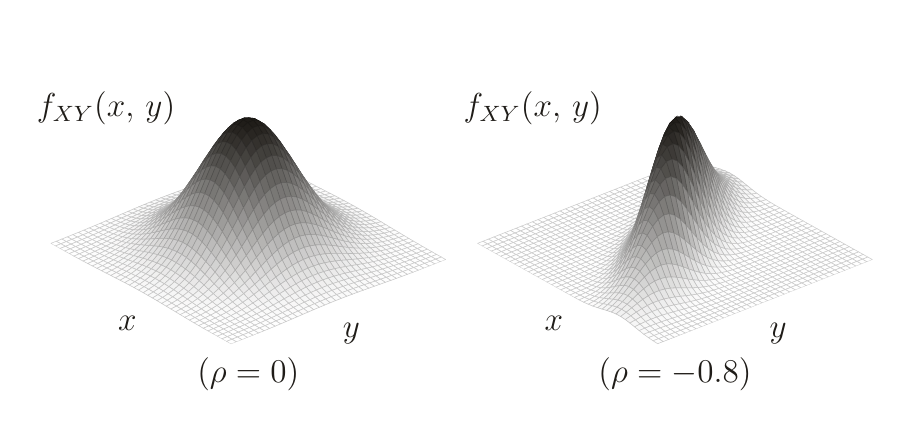
\begin{tikzpicture}[
    declare function={mu1=2;},
    declare function={mu2=2;},
    %% 零相關的那一個: 書稿第 5225 至 5226 行
    declare function={bivarA(\ma,\sa,\mb,\sb)=
        1/(2*pi*\sa*\sb) * exp(-((x-\ma)^2/\sa^2 + (y-\mb)^2/\sb^2))/2;},
    %% 負相關的那一個: 書稿第 5278 至 5279 行
    declare function={bivarB(\ma,\sa,\mb,\sb,\rr)=
        1/(2*pi*\sa*\sb*sqrt(1-\rr^2)) * exp(-((x-\ma)^2/\sa^2 + (y-\mb)^2/\sb^2 - 2*\rr*((x-\ma)/\sa)*((y-\mb)/\sb)))/2;}]
\begin{groupplot}[
  group style={group name=g, group size=2 by 1, horizontal sep=0.4cm},
  surfacepanel,
]

%% 左面板: 相關係數為零，隆起沿兩軸對稱
\nextgroupplot
\addplot3[surf, draw=journalink, line width=0.2pt] {bivarA(mu1,1,mu2,1)};

%% 右面板: 相關係數為負，隆起沿一條斜線拉長
\nextgroupplot
\addplot3[surf, draw=journalink, line width=0.2pt] {bivarB(mu1,0.5,mu2,0.7,-0.8)};

\end{groupplot}

%% 書稿排在 z 軸標示第二行的那一項，改置於各面板正下方
\node[panelnote] at (g c1r1.south) [yshift=-0.05cm] {$(\rho = 0)$};
\node[panelnote] at (g c2r1.south) [yshift=-0.05cm] {$(\rho = -0.8)$};
\end{tikzpicture}
\end{document}
'
%   dvisvgm -O -d2 -n -o ../../images/teaching-topics/bivariate-normal-surface.svg bivariate-normal-surface.dvi

\documentclass[tikz,border=2pt]{standalone}
\usepackage{amsmath}
\usepackage{amssymb}
\usepackage{xcolor}
\usepackage{pgfplots}
\usepgfplotslibrary{groupplots}
\pgfplotsset{compat=1.18}

\definecolor{journalink}{HTML}{1F1C18}
\definecolor{journalmuted}{HTML}{8A7F72}
\definecolor{journalaccent}{HTML}{9C2D2D}

%% 12pt (即 \large) 之下的 script 級撐到 11pt，
%% 使 f 的下標 XY 在 350px 顯示寬之下仍在 11px 之上。
\DeclareMathSizes{12}{12}{11}{10}

%% 書稿用 whitegray 灰階曲面; 本站改用同一色相的墨色濃淡，
%% 與其他圖的主線色 journalink 相稱。
\pgfplotsset{
  colormap={journalgray}{color(0cm)=(white); color(1cm)=(journalink)}
}

\pgfplotsset{
  surfacepanel/.style={
    axis line style={draw=none},
    colormap name=journalgray,
    width=6.6cm,
    height=5.6cm,
    view={50}{45},
    enlargelimits=false,
    domain=0:4,
    y domain=0:4,
    samples=40,
    xlabel=$x$,
    ylabel=$y$,
    zlabel={$f_{XY}(x,\,y)$},
    label style={journalink, font=\large},
    %% 座標軸線設為不畫之後，預設的框線刻度仍會在遠端浮出孤立的短記號，
    %% 一併關掉
    tick style={draw=none},
    xtick=\empty,
    ytick=\empty,
    ztick=\empty,
    zlabel style={rotate=-90, anchor=west, yshift=0.88cm, xshift=-0.30cm},
    xlabel style={yshift=-1.2mm},
    ylabel style={yshift=-1.2mm},
  },
}

\tikzset{panelnote/.style={journalink, font=\large, anchor=north}}

\begin{document}
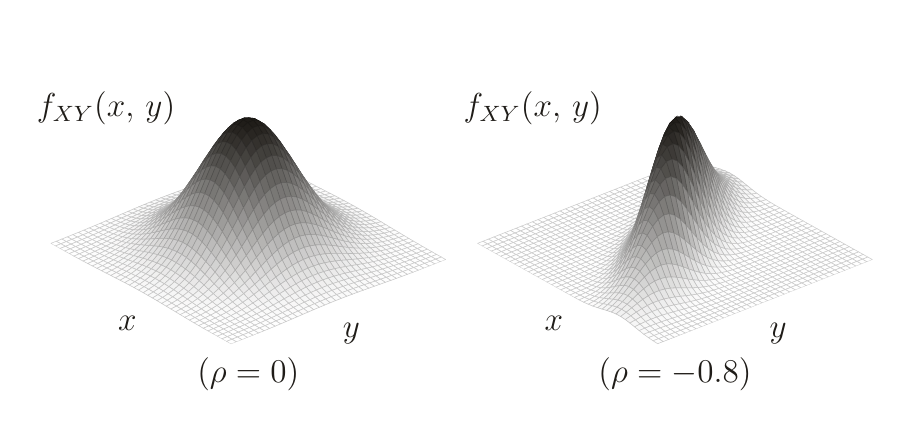
\begin{tikzpicture}[
    declare function={mu1=2;},
    declare function={mu2=2;},
    %% 零相關的那一個: 書稿第 5225 至 5226 行
    declare function={bivarA(\ma,\sa,\mb,\sb)=
        1/(2*pi*\sa*\sb) * exp(-((x-\ma)^2/\sa^2 + (y-\mb)^2/\sb^2))/2;},
    %% 負相關的那一個: 書稿第 5278 至 5279 行
    declare function={bivarB(\ma,\sa,\mb,\sb,\rr)=
        1/(2*pi*\sa*\sb*sqrt(1-\rr^2)) * exp(-((x-\ma)^2/\sa^2 + (y-\mb)^2/\sb^2 - 2*\rr*((x-\ma)/\sa)*((y-\mb)/\sb)))/2;}]
\begin{groupplot}[
  group style={group name=g, group size=2 by 1, horizontal sep=0.4cm},
  surfacepanel,
]

%% 左面板: 相關係數為零，隆起沿兩軸對稱
\nextgroupplot
\addplot3[surf, draw=journalink, line width=0.2pt] {bivarA(mu1,1,mu2,1)};

%% 右面板: 相關係數為負，隆起沿一條斜線拉長
\nextgroupplot
\addplot3[surf, draw=journalink, line width=0.2pt] {bivarB(mu1,0.5,mu2,0.7,-0.8)};

\end{groupplot}

%% 書稿排在 z 軸標示第二行的那一項，改置於各面板正下方
\node[panelnote] at (g c1r1.south) [yshift=-0.05cm] {$(\rho = 0)$};
\node[panelnote] at (g c2r1.south) [yshift=-0.05cm] {$(\rho = -0.8)$};
\end{tikzpicture}
\end{document}
'
%   dvisvgm -O -d2 -n -o ../../images/teaching-topics/bivariate-normal-surface.svg bivariate-normal-surface.dvi

\documentclass[tikz,border=2pt]{standalone}
\usepackage{amsmath}
\usepackage{amssymb}
\usepackage{xcolor}
\usepackage{pgfplots}
\usepgfplotslibrary{groupplots}
\pgfplotsset{compat=1.18}

\definecolor{journalink}{HTML}{1F1C18}
\definecolor{journalmuted}{HTML}{8A7F72}
\definecolor{journalaccent}{HTML}{9C2D2D}

%% 12pt (即 \large) 之下的 script 級撐到 11pt，
%% 使 f 的下標 XY 在 350px 顯示寬之下仍在 11px 之上。
\DeclareMathSizes{12}{12}{11}{10}

%% 書稿用 whitegray 灰階曲面; 本站改用同一色相的墨色濃淡，
%% 與其他圖的主線色 journalink 相稱。
\pgfplotsset{
  colormap={journalgray}{color(0cm)=(white); color(1cm)=(journalink)}
}

\pgfplotsset{
  surfacepanel/.style={
    axis line style={draw=none},
    colormap name=journalgray,
    width=6.6cm,
    height=5.6cm,
    view={50}{45},
    enlargelimits=false,
    domain=0:4,
    y domain=0:4,
    samples=40,
    xlabel=$x$,
    ylabel=$y$,
    zlabel={$f_{XY}(x,\,y)$},
    label style={journalink, font=\large},
    %% 座標軸線設為不畫之後，預設的框線刻度仍會在遠端浮出孤立的短記號，
    %% 一併關掉
    tick style={draw=none},
    xtick=\empty,
    ytick=\empty,
    ztick=\empty,
    zlabel style={rotate=-90, anchor=west, yshift=0.88cm, xshift=-0.30cm},
    xlabel style={yshift=-1.2mm},
    ylabel style={yshift=-1.2mm},
  },
}

\tikzset{panelnote/.style={journalink, font=\large, anchor=north}}

\begin{document}
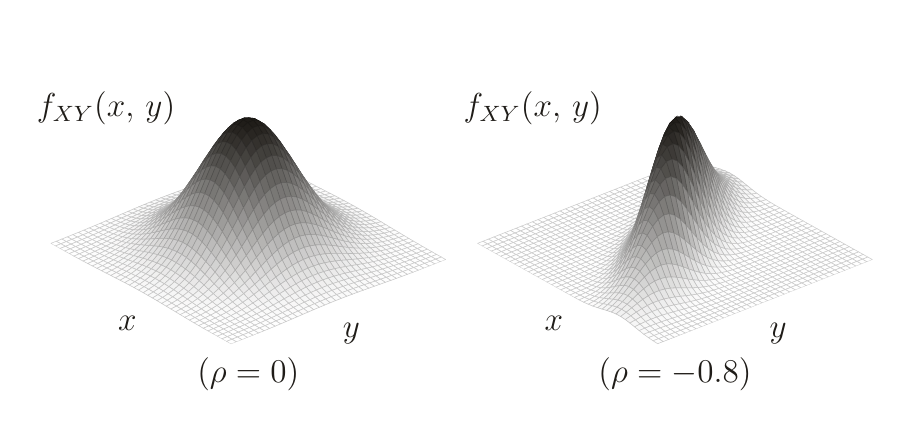
\begin{tikzpicture}[
    declare function={mu1=2;},
    declare function={mu2=2;},
    %% 零相關的那一個: 書稿第 5225 至 5226 行
    declare function={bivarA(\ma,\sa,\mb,\sb)=
        1/(2*pi*\sa*\sb) * exp(-((x-\ma)^2/\sa^2 + (y-\mb)^2/\sb^2))/2;},
    %% 負相關的那一個: 書稿第 5278 至 5279 行
    declare function={bivarB(\ma,\sa,\mb,\sb,\rr)=
        1/(2*pi*\sa*\sb*sqrt(1-\rr^2)) * exp(-((x-\ma)^2/\sa^2 + (y-\mb)^2/\sb^2 - 2*\rr*((x-\ma)/\sa)*((y-\mb)/\sb)))/2;}]
\begin{groupplot}[
  group style={group name=g, group size=2 by 1, horizontal sep=0.4cm},
  surfacepanel,
]

%% 左面板: 相關係數為零，隆起沿兩軸對稱
\nextgroupplot
\addplot3[surf, draw=journalink, line width=0.2pt] {bivarA(mu1,1,mu2,1)};

%% 右面板: 相關係數為負，隆起沿一條斜線拉長
\nextgroupplot
\addplot3[surf, draw=journalink, line width=0.2pt] {bivarB(mu1,0.5,mu2,0.7,-0.8)};

\end{groupplot}

%% 書稿排在 z 軸標示第二行的那一項，改置於各面板正下方
\node[panelnote] at (g c1r1.south) [yshift=-0.05cm] {$(\rho = 0)$};
\node[panelnote] at (g c2r1.south) [yshift=-0.05cm] {$(\rho = -0.8)$};
\end{tikzpicture}
\end{document}
'
%   dvisvgm -O -d2 -n -o ../../images/teaching-topics/bivariate-normal-surface.svg bivariate-normal-surface.dvi

\documentclass[tikz,border=2pt]{standalone}
\usepackage{amsmath}
\usepackage{amssymb}
\usepackage{xcolor}
\usepackage{pgfplots}
\usepgfplotslibrary{groupplots}
\pgfplotsset{compat=1.18}

\definecolor{journalink}{HTML}{1F1C18}
\definecolor{journalmuted}{HTML}{8A7F72}
\definecolor{journalaccent}{HTML}{9C2D2D}

%% 12pt (即 \large) 之下的 script 級撐到 11pt，
%% 使 f 的下標 XY 在 350px 顯示寬之下仍在 11px 之上。
\DeclareMathSizes{12}{12}{11}{10}

%% 書稿用 whitegray 灰階曲面; 本站改用同一色相的墨色濃淡，
%% 與其他圖的主線色 journalink 相稱。
\pgfplotsset{
  colormap={journalgray}{color(0cm)=(white); color(1cm)=(journalink)}
}

\pgfplotsset{
  surfacepanel/.style={
    axis line style={draw=none},
    colormap name=journalgray,
    width=6.6cm,
    height=5.6cm,
    view={50}{45},
    enlargelimits=false,
    domain=0:4,
    y domain=0:4,
    samples=40,
    xlabel=$x$,
    ylabel=$y$,
    zlabel={$f_{XY}(x,\,y)$},
    label style={journalink, font=\large},
    %% 座標軸線設為不畫之後，預設的框線刻度仍會在遠端浮出孤立的短記號，
    %% 一併關掉
    tick style={draw=none},
    xtick=\empty,
    ytick=\empty,
    ztick=\empty,
    zlabel style={rotate=-90, anchor=west, yshift=0.88cm, xshift=-0.30cm},
    xlabel style={yshift=-1.2mm},
    ylabel style={yshift=-1.2mm},
  },
}

\tikzset{panelnote/.style={journalink, font=\large, anchor=north}}

\begin{document}
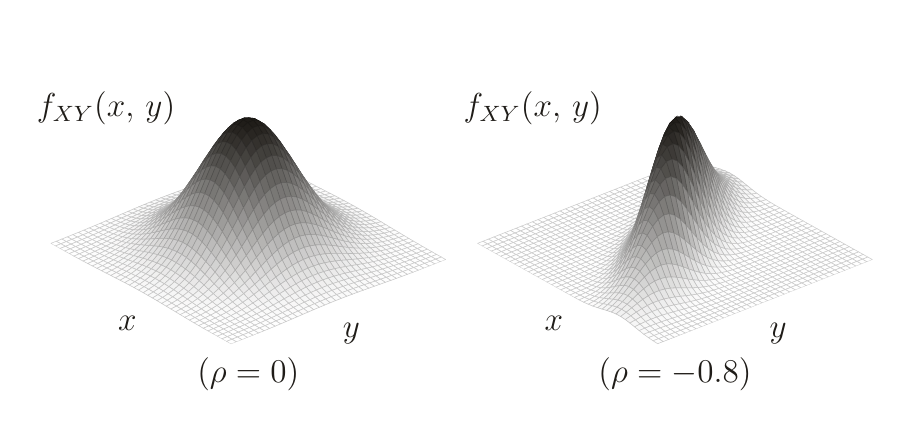
\begin{tikzpicture}[
    declare function={mu1=2;},
    declare function={mu2=2;},
    %% 零相關的那一個: 書稿第 5225 至 5226 行
    declare function={bivarA(\ma,\sa,\mb,\sb)=
        1/(2*pi*\sa*\sb) * exp(-((x-\ma)^2/\sa^2 + (y-\mb)^2/\sb^2))/2;},
    %% 負相關的那一個: 書稿第 5278 至 5279 行
    declare function={bivarB(\ma,\sa,\mb,\sb,\rr)=
        1/(2*pi*\sa*\sb*sqrt(1-\rr^2)) * exp(-((x-\ma)^2/\sa^2 + (y-\mb)^2/\sb^2 - 2*\rr*((x-\ma)/\sa)*((y-\mb)/\sb)))/2;}]
\begin{groupplot}[
  group style={group name=g, group size=2 by 1, horizontal sep=0.4cm},
  surfacepanel,
]

%% 左面板: 相關係數為零，隆起沿兩軸對稱
\nextgroupplot
\addplot3[surf, draw=journalink, line width=0.2pt] {bivarA(mu1,1,mu2,1)};

%% 右面板: 相關係數為負，隆起沿一條斜線拉長
\nextgroupplot
\addplot3[surf, draw=journalink, line width=0.2pt] {bivarB(mu1,0.5,mu2,0.7,-0.8)};

\end{groupplot}

%% 書稿排在 z 軸標示第二行的那一項，改置於各面板正下方
\node[panelnote] at (g c1r1.south) [yshift=-0.05cm] {$(\rho = 0)$};
\node[panelnote] at (g c2r1.south) [yshift=-0.05cm] {$(\rho = -0.8)$};
\end{tikzpicture}
\end{document}
